%
% Experiments
%
\chapter{Experiments} \label{sec:experiments}
In this chapter we will perform experiments to investigate to what extent the methods proposed in Chapter \ref{sec:methodology} can improve the performance of VGC-Bench's RL agents under non-stationarity.
We do this in three phases:

\begin{enumerate}
    \item \textbf{Stationary Experiments:} We train progressive and tuned PPO agents from scratch on each regulation and evaluate using 1000 episodes of cross-play, both in-distribution and out-of-distribution, against the original VGC-Bench RL agents. This experiment will show us what effect a progressive architecture and tuned PPO have on the performance and generalization of agents in a stationary environment.
    \item \textbf{Non-Stationary Experiments:} We transfer the agents trained on regulation \textbf{A} to regulation \textbf{B}, then \textbf{C}, etc. using the progressive architecture, full fine-tuning using tuned PPO, and a combination of the two. We evaluate using 1000 episodes of cross-play, both in-distribution and out-of-distribution, against the original fine-tuned agents and agents trained from scratch. This experiment will show us what effect a progressive architecture and tuned PPO have on the performance and generalization of agents in a non-stationary setting.
    \item \textbf{Analysis Experiments:} To further analyze the effects of a progressive architecture and tuned PPO, we will also repeat the action probabilities, value function, and action logits experiments performed in Chapter \ref{sec:preliminary:analysis}.
\end{enumerate}

All agents are implemented as outlined in Chapter \ref{sec:methodology} and trained using the default hyperparameters shown in Table \ref{tab:hyperparam-vgcbench}, unless otherwise stated.
Just as in Chapter \ref{sec:preliminary}, regulations \textbf{B}, \textbf{E}, and \textbf{J} are excluded from out-of-distribution results because there are not enough teams available for a full out-of-distribution set.

\section{Stationary Results} \label{sec:results:stationary}
We train progressive and tuned PPO agents on all regulations.
Evaluation is done, both in-distribution and out-of-distribution, using 1000 episodes of cross-play against each other and against the original, unmodified VGC-Bench agents.
The results are shown in Figure \ref{fig:stationary}.

\begin{figure}[H]
    \centering
    \begin{subfigure}{\textwidth}
        \centering
        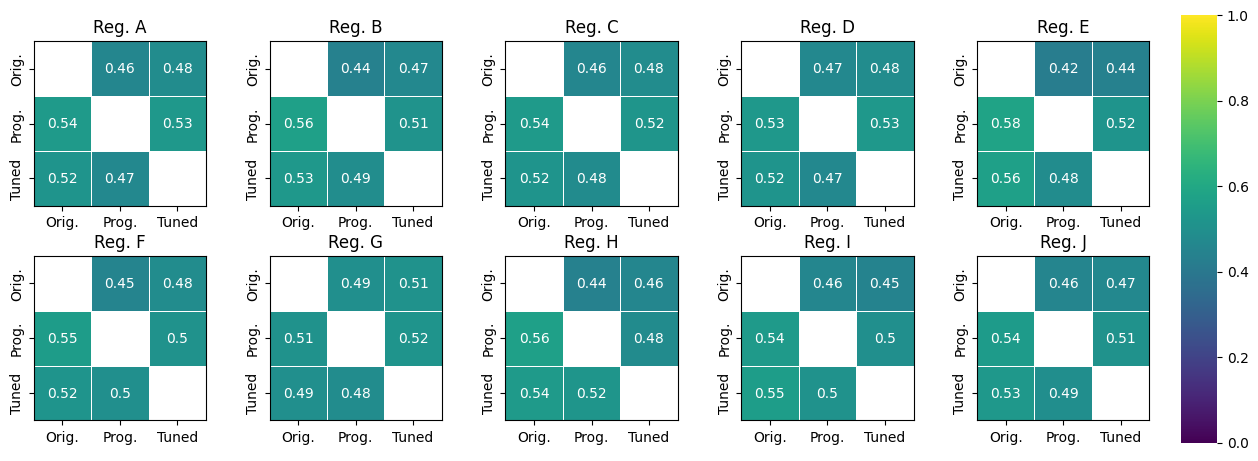
\includegraphics[width=\textwidth]{images/experiments/stationary-indist.png}
        \caption{In-distribution.}
        \label{fig:stationary-indist}
    \end{subfigure}
    \par\bigskip
    \begin{subfigure}{.85\textwidth}
        \centering
        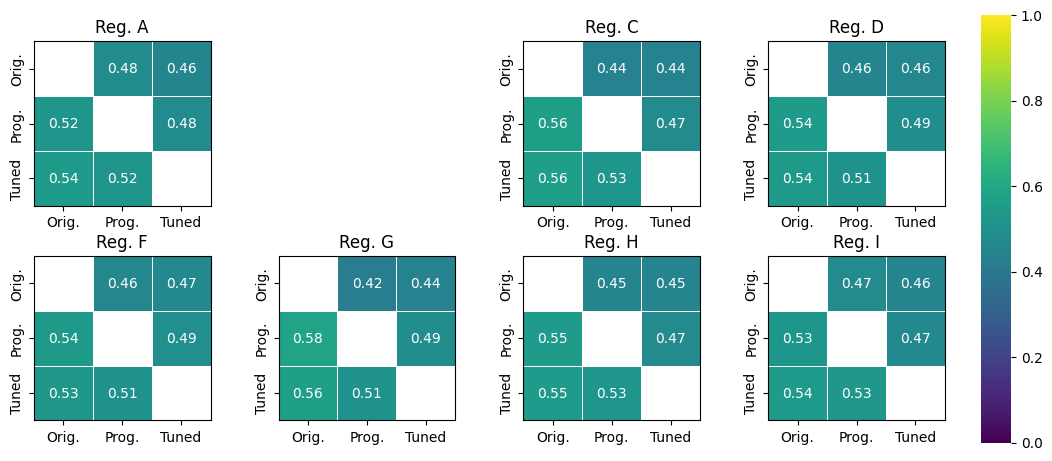
\includegraphics[width=\textwidth]{images/experiments/stationary-outofdist.png}
        \caption{Out-of-distribution.}
        \label{fig:stationary-outdist}
    \end{subfigure}
    \caption{Win rates of the row player over 1000 episodes in each regulation. \textit{``Orig."} refers to the original, unmodified agents from VGC-Bench, \textit{``Prog."} refers to agents trained with a progressive architecture, \textit{``Tuned"} refers to agents trained using tuned PPO.}
    \label{fig:stationary}
\end{figure}

We define our null hypothesis $H_0$ to be that an agent $\phi$ is equally skilled or worse than an agent $\psi$, and we define our significance level to be $\alpha=0.05$.
Just as in Chapter \ref{sec:preliminary}, we use a Binomial test with $n=1000$ and an expected win rate of $p \leq 0.5$ to calculate the p-values of the win rates of agent $\phi$.
These p-values are shown in Figure \ref{fig:stationary-pvalues}.

\begin{figure}[H]
    \centering
    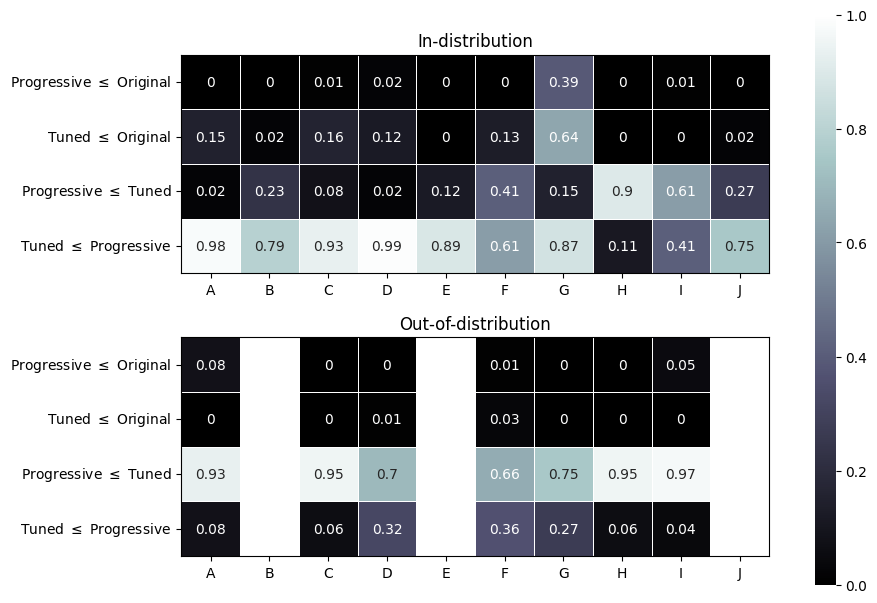
\includegraphics[width=0.9\textwidth]{images/experiments/stationary-pvalues.png}
    \caption{P-values of the win rates of the left agent against the right agent (e.g. the top row shows the p-values of the win rates of the agent with a progressive architecture against the original agent, belonging to the null hypothesis that the former is equally skilled or worse than the latter). Letters on the horizontal axis represent the regulation the agents are trained and evaluated on.}
    \label{fig:stationary-pvalues}
\end{figure}

\section{Non-Stationary Results} \label{sec:results:nonstationary}
We transfer the agents trained on regulation \textbf{A} to regulation \textbf{B}, then \textbf{C}, etc. using the progressive architecture (\textit{``progressive agents"}), full fine-tuning using tuned PPO (\textit{``tuned agents"}), and a combination of both (\textit{``combined agents"}).
Additional training or fine-tuning is always done for the same number of steps as training from scratch to provide an upper bound of the expected performance, and using the same hyperparameters as regular training (excluding tuned PPO, as outlined in Chapter \ref{sec:tuned}).
We evaluate using 1000 episodes of cross-play, both in-distribution and out-of-distribution, against the original fine-tuned agents and agents trained from scratch.

The results for the progressive, tuned, and combined agents are shown in Figures \ref{fig:progressive-experiments}, \ref{fig:tuned-experiments}, and \ref{fig:combined-experiments} respectively.
Additionally, results showing how the three types of agents compare against each other are shown in Figure \ref{fig:compared-experiments}.
Using the same null hypothesis, significance level, and statistical test as in Chapter \ref{sec:results:stationary}, the p-values of the win rates of the progressive, tuned, and combined agents are shown in Figures \ref{fig:progressive-pvalues}, \ref{fig:tuned-pvalues}, and \ref{fig:combined-pvalues} respectively.

\begin{figure}[ht]
    \centering
    \begin{subfigure}{.5\textwidth}
        \centering
        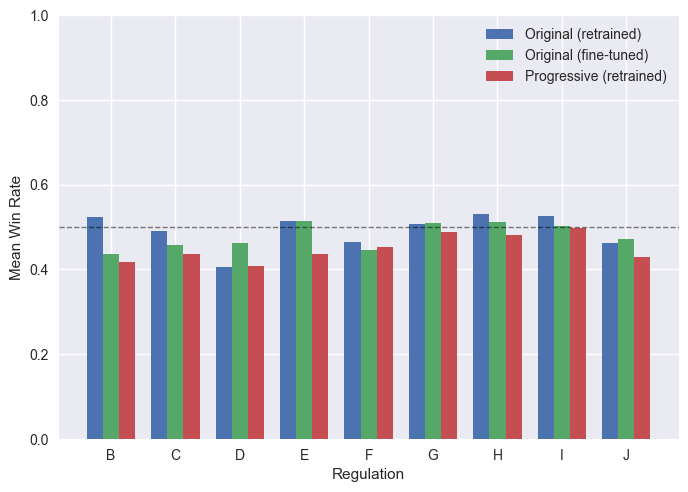
\includegraphics[width=\textwidth]{images/experiments/progressive-indist.png}
        \caption{In-distribution.}
        \label{fig:progressive-indist}
    \end{subfigure}%
    \begin{subfigure}{.5\textwidth}
        \centering
        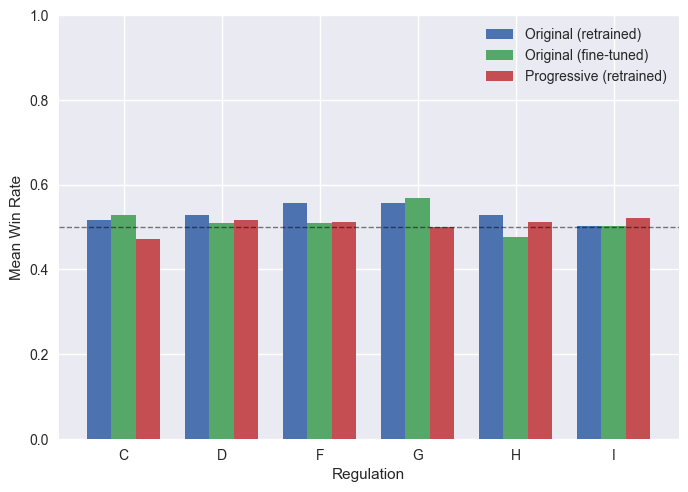
\includegraphics[width=\textwidth]{images/experiments/progressive-outofdist.png}
        \caption{Out-of-distribution.}
        \label{fig:progressive-outofdist}
    \end{subfigure}
    \caption{Mean win rates of progressive agents against VGC-Bench's original agents trained from scratch (blue), VGC-Bench's original agents fine-tuned (green), and progressive agents trained from scratch (red). Evaluated over 1000 episodes on each regulation.}
    \label{fig:progressive-experiments}
\end{figure}

\begin{figure}[ht]
    \centering
    \begin{subfigure}{.5\textwidth}
        \centering
        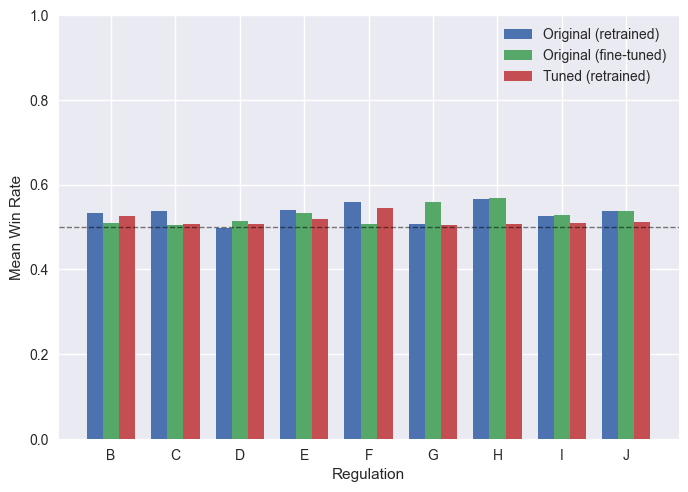
\includegraphics[width=\textwidth]{images/experiments/tuned-indist.png}
        \caption{In-distribution.}
        \label{fig:tuned-indist}
    \end{subfigure}%
    \begin{subfigure}{.5\textwidth}
        \centering
        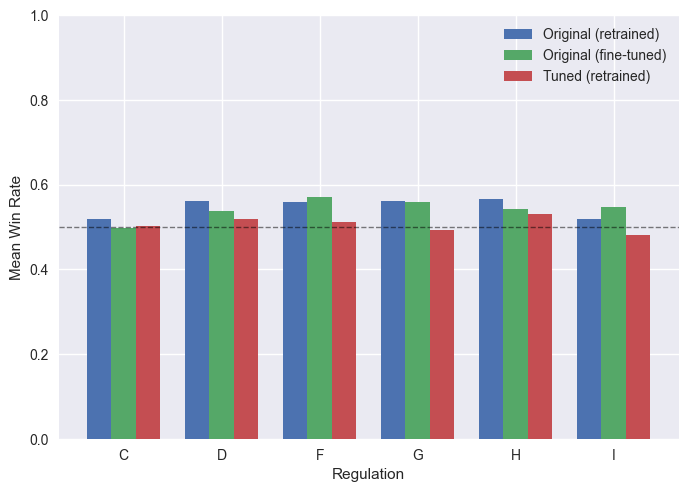
\includegraphics[width=\textwidth]{images/experiments/tuned-outofdist.png}
        \caption{Out-of-distribution.}
        \label{fig:tuned-outofdist}
    \end{subfigure}
    \caption{Mean win rates of tuned agents against VGC-Bench's original agents trained from scratch (blue), VGC-Bench's original agents fine-tuned (green), and tuned agents trained from scratch (red). Evaluated over 1000 episodes on each regulation.}
    \label{fig:tuned-experiments}
\end{figure}

\begin{figure}[ht]
    \centering
    \begin{subfigure}{.5\textwidth}
        \centering
        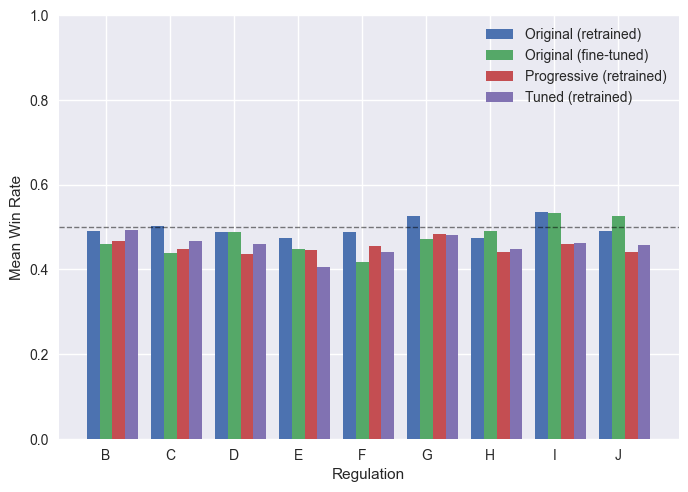
\includegraphics[width=\textwidth]{images/experiments/combined-indist.png}
        \caption{In-distribution.}
        \label{fig:combined-indist}
    \end{subfigure}%
    \begin{subfigure}{.5\textwidth}
        \centering
        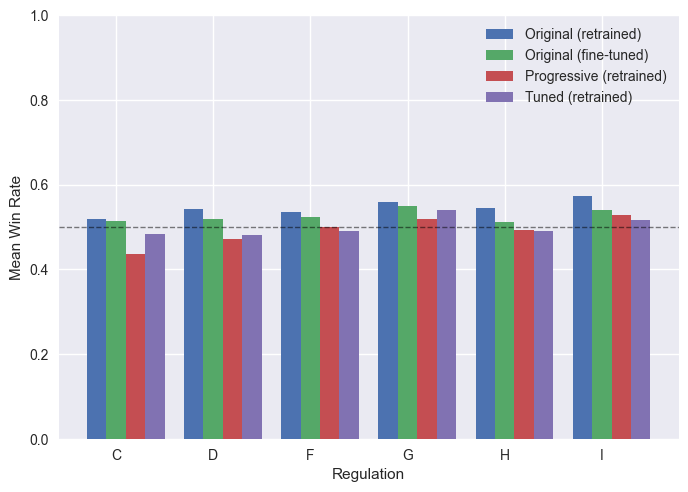
\includegraphics[width=\textwidth]{images/experiments/combined-outofdist.png}
        \caption{Out-of-distribution.}
        \label{fig:combined-outofdist}
    \end{subfigure}
    \caption{Mean win rates of combined agents against VGC-Bench's original agents trained from scratch (blue), VGC-Bench's original agents fine-tuned (green), progressive agents trained from scratch (red), and tuned agents trained from scratch (purple). Evaluated over 1000 episodes on each regulation.}
    \label{fig:combined-experiments}
\end{figure}

\begin{figure}[ht]
    \centering
    \begin{subfigure}{0.9\textwidth}
        \centering
        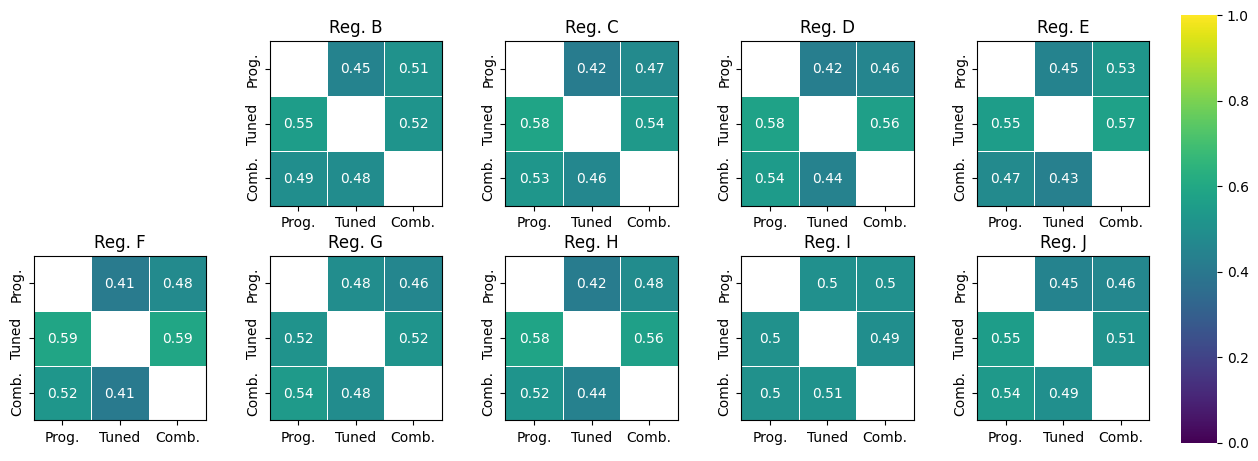
\includegraphics[width=\textwidth]{images/experiments/compared-indist.png}
        \caption{In-distribution.}
        \label{fig:compared-indist}
    \end{subfigure}
    \par\bigskip
    \begin{subfigure}{.55\textwidth}
        \centering
        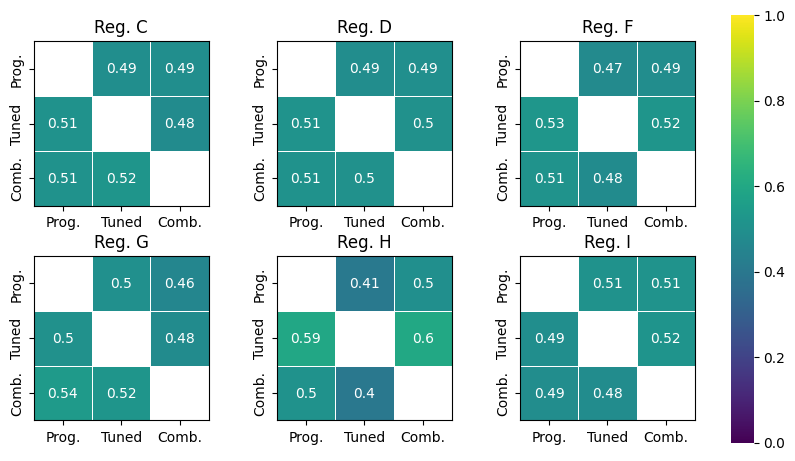
\includegraphics[width=\textwidth]{images/experiments/compared-outofdist.png}
        \caption{Out-of-distribution.}
        \label{fig:compared-outdist}
    \end{subfigure}
    \caption{Win rates of the row player over 1000 episodes in each regulation. \textit{``Prog."} refers to progressive agents, \textit{``Tuned"} refers to tuned agents, \textit{``Comb."} refers to combined agents.}
    \label{fig:compared-experiments}
\end{figure}

\begin{figure}[ht]
    \centering
    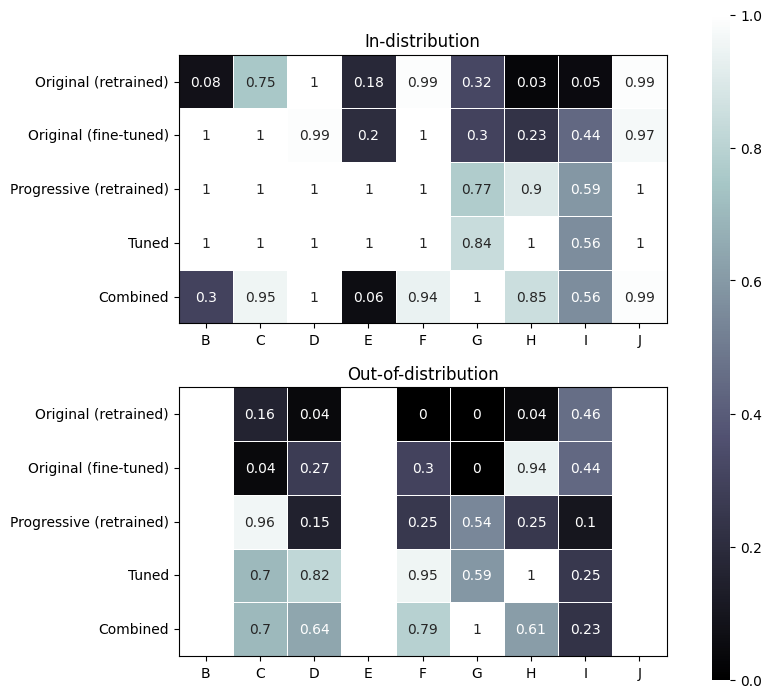
\includegraphics[width=\textwidth]{images/experiments/progressive-pvalues.png}
    \caption{P-values of the win rates of progressive agents against the agents on the vertical axis, in the regulation on the horizontal axis.}
    \label{fig:progressive-pvalues}
\end{figure}

\begin{figure}[ht]
    \centering
    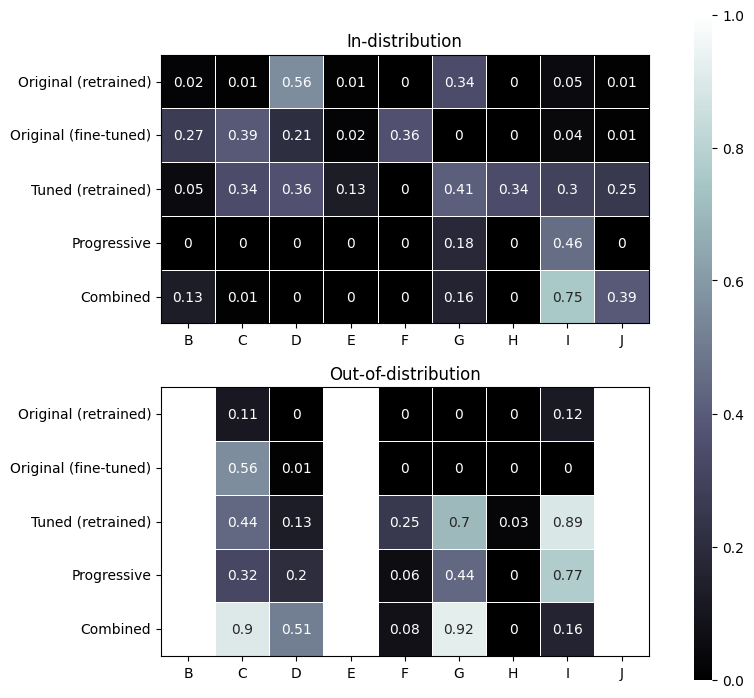
\includegraphics[width=\textwidth]{images/experiments/tuned-pvalues.png}
    \caption{P-values of the win rates of the tuned agents against the agents on the vertical axis, in the regulation on the horizontal axis.}
    \label{fig:tuned-pvalues}
\end{figure}

\begin{figure}[ht]
    \centering
    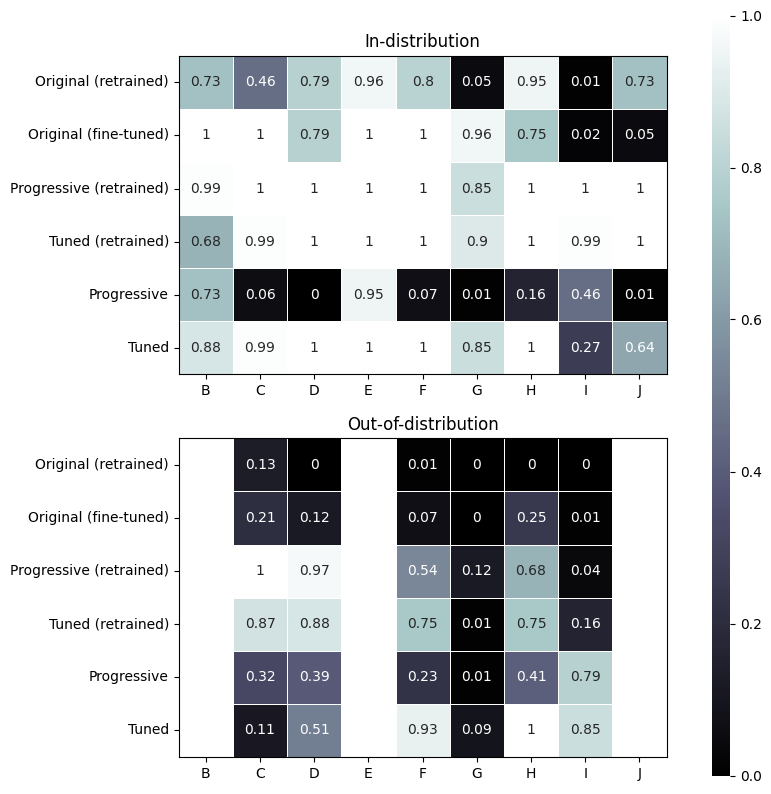
\includegraphics[width=\textwidth]{images/experiments/combined-pvalues.png}
    \caption{P-values of the win rates of the combined agents against the agents on the vertical axis, in the regulation on the horizontal axis.}
    \label{fig:combined-pvalues}
\end{figure}

\FloatBarrier

\section{Analysis Results} \label{sec:results:analysis}
Just as in Chapter \ref{sec:preliminary:analysis}, we further analyze our agents in regulations \textbf{F} and \textbf{G} by running 100 episodes of cross-play, both in-distribution and out-of-distribution, collecting statistics such as action probabilities, action logits, and value predictions for every observation.
We do this for the progressive agent trained on the regulation from scratch, the progressive and tuned agents fine-tuned up to the regulation, and the progressive and tuned agents fine-tuned up to the previous regulation.
We omit the combined agent from these experiments as we are more interested in analyzing the methods individually.

The first experiment focuses on how similar the agents are in their decision making, which we measure as the Jensen-Shannon distance between their respective action probabilities.
The results are shown in Figure \ref{fig:jsd-experiments}.

\begin{figure}[H]
    \centering
    \begin{subfigure}{.475\textwidth}
        \centering
        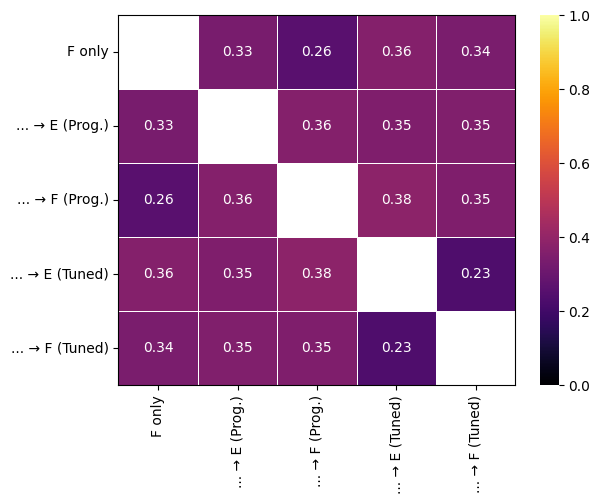
\includegraphics[width=\textwidth]{images/experiments/jsd-regf-indist.png}
        \caption{Regulation \textbf{F}, in-distribution ($n=924$).}
        \label{fig:jsd-experiments-regf-indist}
    \end{subfigure}
    \hfill
    \begin{subfigure}{.475\textwidth}
        \centering
        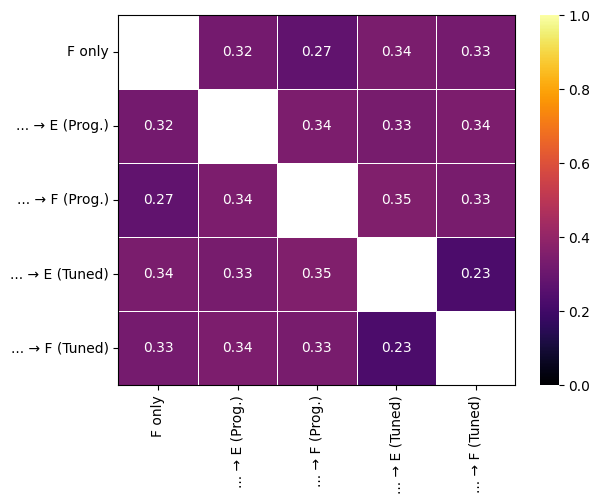
\includegraphics[width=\textwidth]{images/experiments/jsd-regf-outofdist.png}
        \caption{Regulation \textbf{F}, out-of-distribution ($n=1021$).}
        \label{fig:jsd-experiments-regf-outdist}
    \end{subfigure}
    \vskip\baselineskip
    \begin{subfigure}{.475\textwidth}
        \centering
        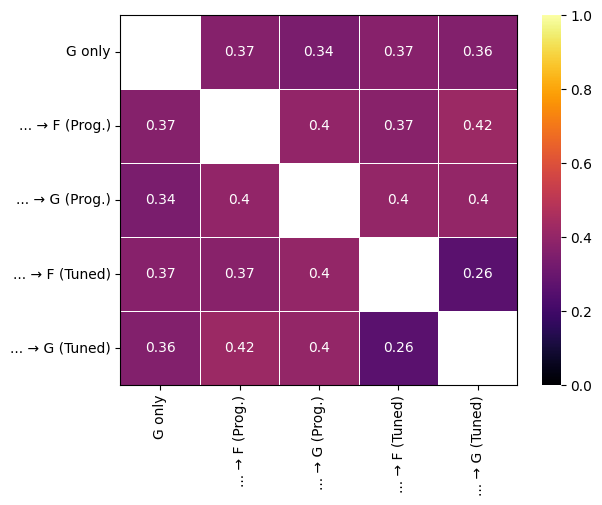
\includegraphics[width=\textwidth]{images/experiments/jsd-regg-indist.png}
        \caption{Regulation \textbf{G}, in-distribution ($n=1041$).}
        \label{fig:jsd-experiments-regg-indist}
    \end{subfigure}
    \hfill
    \begin{subfigure}{.475\textwidth}
        \centering
        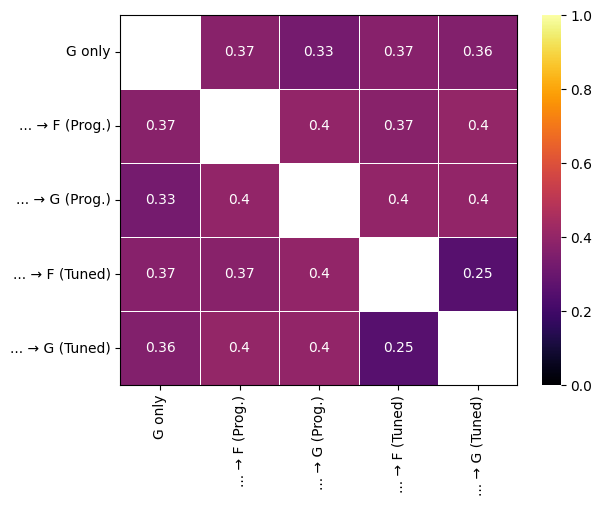
\includegraphics[width=\textwidth]{images/experiments/jsd-regg-outofdist.png}
        \caption{Regulation \textbf{G}, out-of-distribution ($n=1012$).}
        \label{fig:jsd-experiments-regg-outdist}
    \end{subfigure}
    \caption{Mean pairwise Jensen-Shannon distance between action probabilities for every observation. Letters represent the regulation the agent is trained or fine-tuned on (e.g. ``$... \rightarrow \text{F}$" is fine-tuned from regulation \textbf{A} to \textbf{B} to ... to \textbf{F}). \textit{``Prog."} refers to progressive agents.}
    \label{fig:jsd-experiments}
\end{figure}

In the next experiment we compare the value predictions of the agents when given the same observation.
The results for this experiment, plotted against the normalized depth of the observation (how many turns into the battle it was recorded), are shown in Figure \ref{fig:value-experiments}.

\begin{figure}[H]
    \centering
    \begin{subfigure}{.5\textwidth}
        \centering
        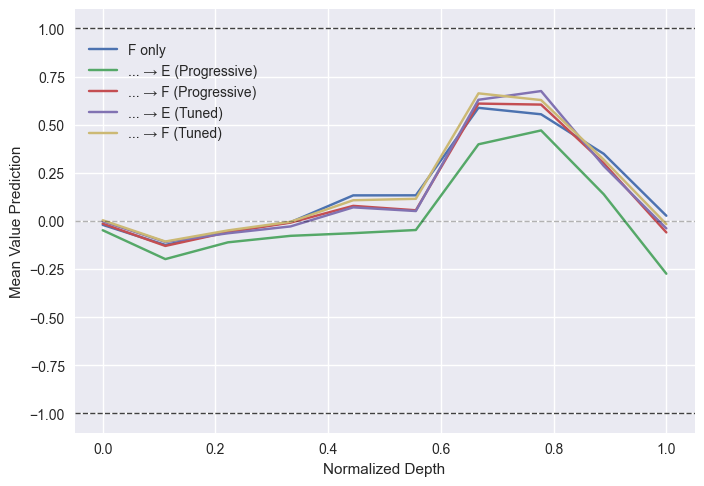
\includegraphics[width=\textwidth]{images/experiments/value-regf-indist.png}
        \caption{Regulation \textbf{F}, in-distribution ($n=924$).}
        \label{fig:value-experiments-regf-indist}
    \end{subfigure}%
    \begin{subfigure}{.5\textwidth}
        \centering
        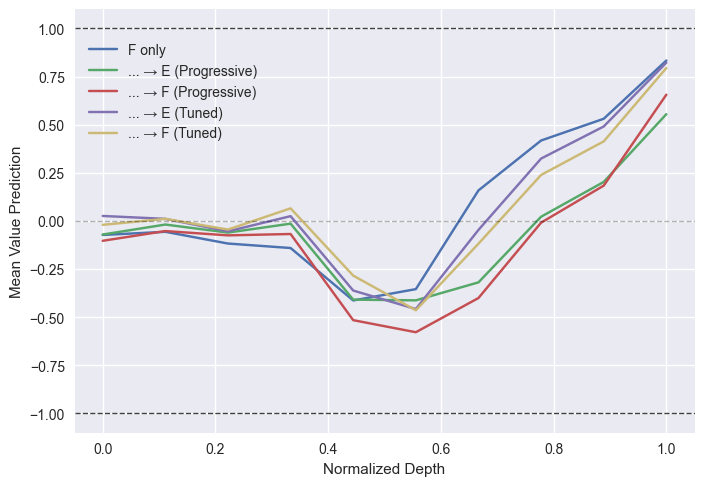
\includegraphics[width=\textwidth]{images/experiments/value-regf-outofdist.png}
        \caption{Regulation \textbf{F}, out-of-distribution ($n=1021$).}
        \label{fig:value-experiments-regf-outdist}
    \end{subfigure}
    \vskip\baselineskip
    \begin{subfigure}{.5\textwidth}
        \centering
        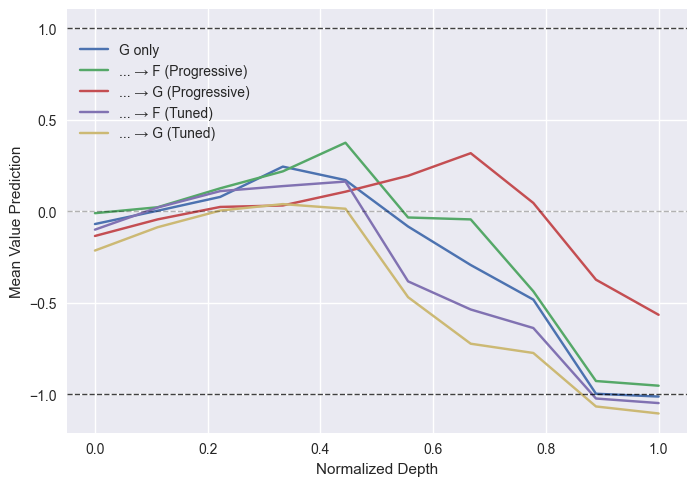
\includegraphics[width=\textwidth]{images/experiments/value-regg-indist.png}
        \caption{Regulation \textbf{G}, in-distribution ($n=1041$).}
        \label{fig:value-experiments-regg-indist}
    \end{subfigure}%
    \begin{subfigure}{.5\textwidth}
        \centering
        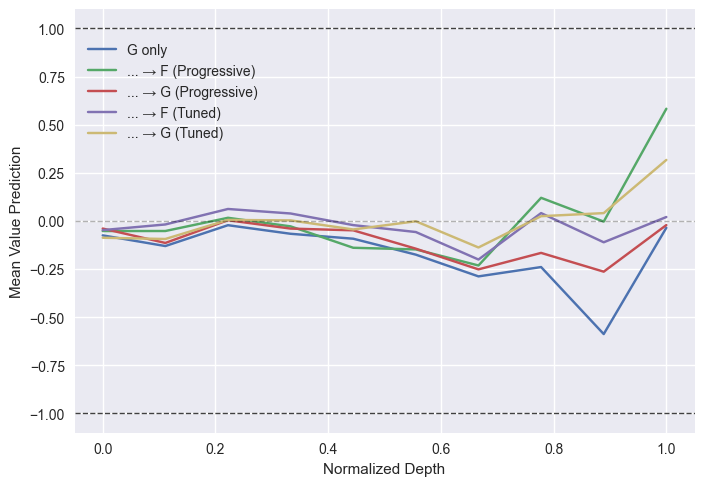
\includegraphics[width=\textwidth]{images/experiments/value-regg-outofdist.png}
        \caption{Regulation \textbf{G}, out-of-distribution ($n=1012$).}
        \label{fig:value-experiments-regg-outdist}
    \end{subfigure}
    \caption{Mean value prediction for every observation, plotted against the normalized depth. Letters represent the regulation the agent is trained or fine-tuned on (e.g. ``$... \rightarrow \text{F}$" is fine-tuned from regulation \textbf{A} to \textbf{B} to ... to \textbf{F}).}
    \label{fig:value-experiments}
\end{figure}

The last experiment involves plotting the distribution of action logits using a t-SNE visualization.
Just as in Chapter \ref{sec:preliminary:analysis}, we take the 256-dimensional action logits for each observation, reduce them to 50 dimensions using principal component analysis (PCA), then reduce them to two dimensions using t-SNE.
The visualizations for progressive and tuned agents can be found in Figures \ref{fig:tsne-progressive} and \ref{fig:tsne-tuned} respectively.

To get a clearer picture of the underlying structure of the latter visualization, we sample 50 observations (150 points) and connect points showing logits of the same observation.
Since t-SNE distorts global and local distances, we color these connecting lines according to the Jensen-Shannon distance between the action probabilities of the respective observations.
This visualization can be found in Figure \ref{fig:tsne-tuned-lines}.

\begin{figure}[ht]
    \centering
    \begin{subfigure}{.5\textwidth}
        \centering
        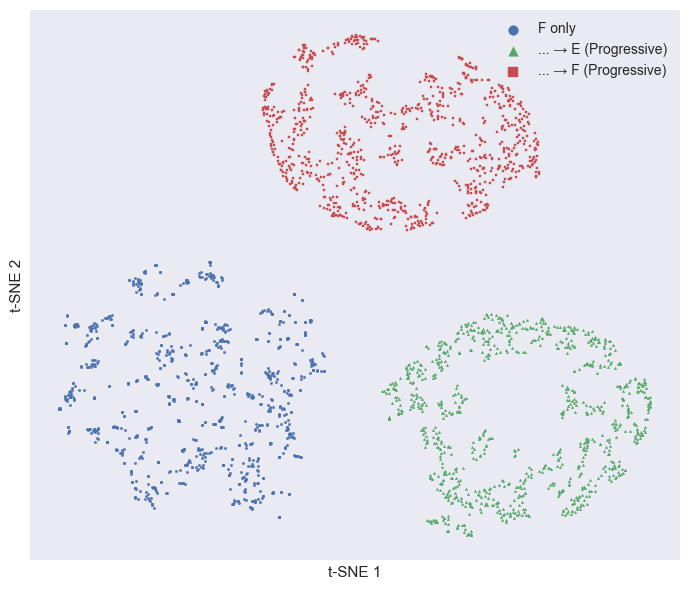
\includegraphics[width=\textwidth]{images/experiments/progressive-tsne-regf-indist.png}
        \caption{Regulation \textbf{F}, in-distribution ($n=924$).}
        \label{fig:tsne-progressive-regf-indist}
    \end{subfigure}%
    \begin{subfigure}{.5\textwidth}
        \centering
        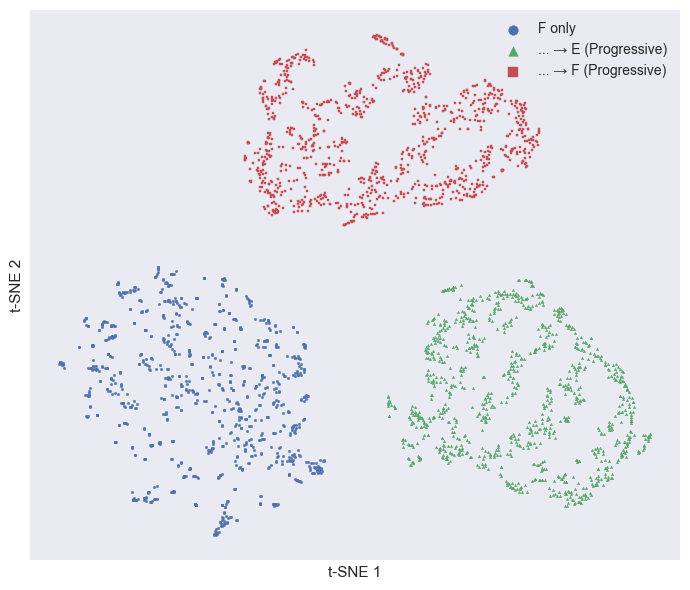
\includegraphics[width=\textwidth]{images/experiments/progressive-tsne-regf-outofdist.png}
        \caption{Regulation \textbf{F}, out-of-distribution ($n=1021$).}
        \label{fig:tsne-progressive-regf-outdist}
    \end{subfigure}
    \vskip\baselineskip
    \begin{subfigure}{.5\textwidth}
        \centering
        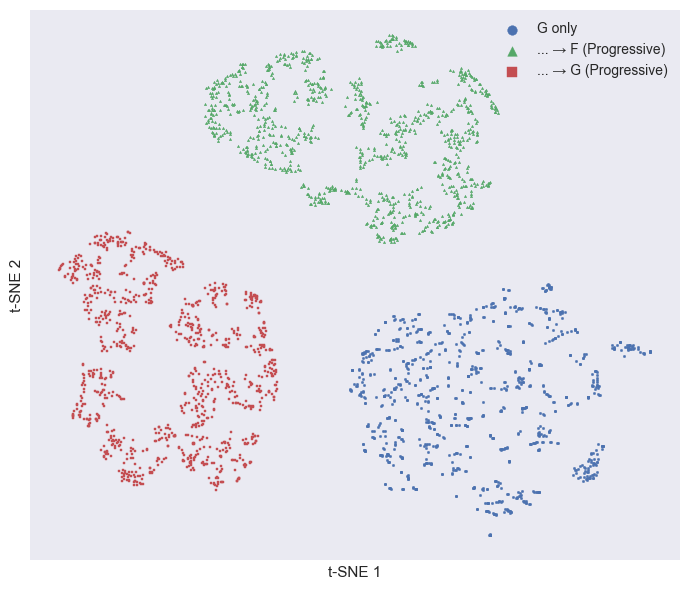
\includegraphics[width=\textwidth]{images/experiments/progressive-tsne-regg-indist.png}
        \caption{Regulation \textbf{G}, in-distribution ($n=1041$).}
        \label{fig:tsne-progressive-regg-indist}
    \end{subfigure}%
    \begin{subfigure}{.5\textwidth}
        \centering
        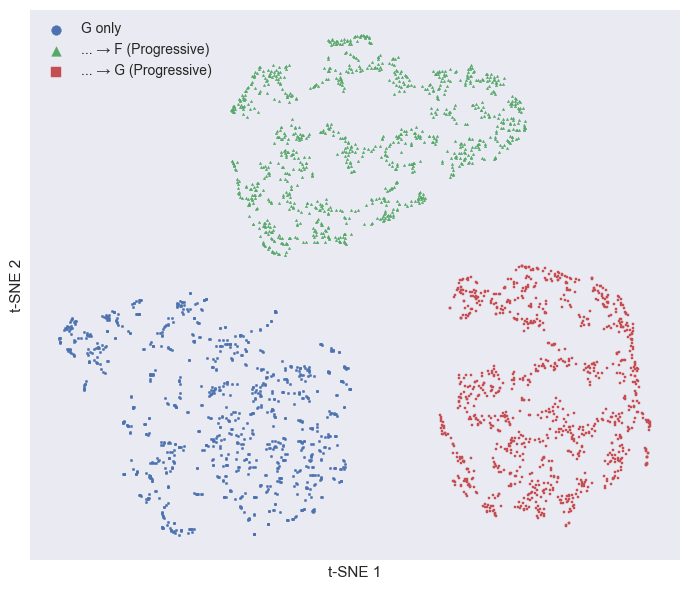
\includegraphics[width=\textwidth]{images/experiments/progressive-tsne-regg-outofdist.png}
        \caption{Regulation \textbf{G}, out-of-distribution ($n=1012$).}
        \label{fig:tsne-progressive-regg-outdist}
    \end{subfigure}
    \caption{t-SNE visualization of action logits of progressive agents for every observation. Letters represent the regulation the agent is trained or fine-tuned on (e.g. ``$... \rightarrow \text{F}$" is fine-tuned from regulation \textbf{A} to \textbf{B} to ... to \textbf{F}).}
    \label{fig:tsne-progressive}
\end{figure}

\begin{figure}[ht]
    \centering
    \begin{subfigure}{.5\textwidth}
        \centering
        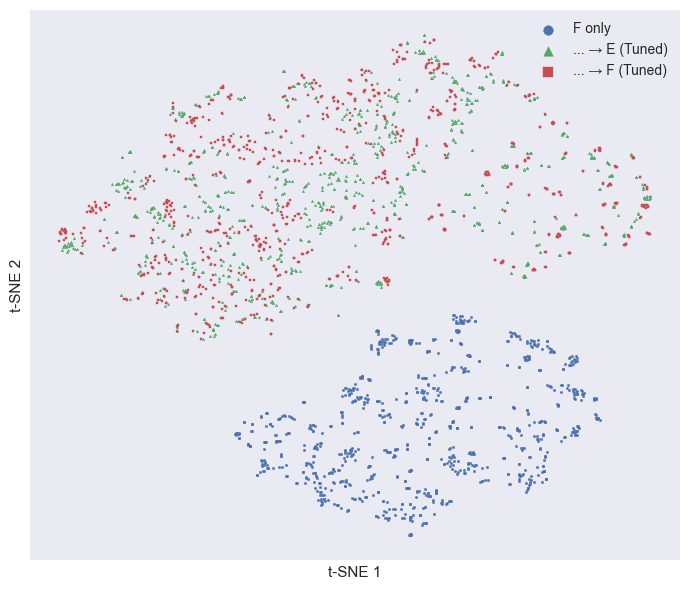
\includegraphics[width=\textwidth]{images/experiments/tuned-tsne-regf-indist.png}
        \caption{Regulation \textbf{F}, in-distribution ($n=924$).}
        \label{fig:tsne-tuned-regf-indist}
    \end{subfigure}%
    \begin{subfigure}{.5\textwidth}
        \centering
        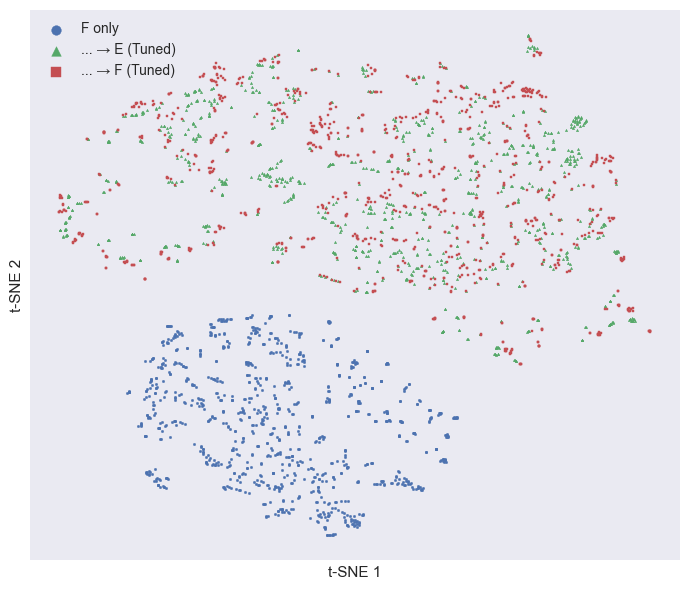
\includegraphics[width=\textwidth]{images/experiments/tuned-tsne-regf-outofdist.png}
        \caption{Regulation \textbf{F}, out-of-distribution ($n=1021$).}
        \label{fig:tsne-tuned-regf-outdist}
    \end{subfigure}
    \vskip\baselineskip
    \begin{subfigure}{.5\textwidth}
        \centering
        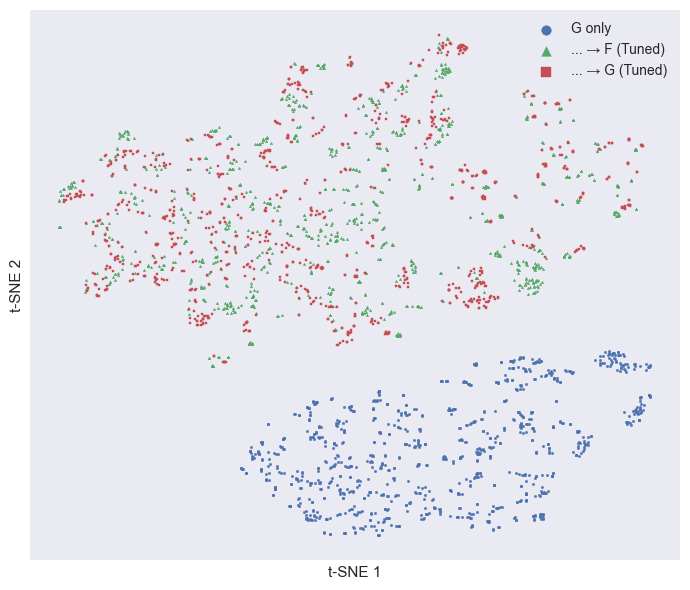
\includegraphics[width=\textwidth]{images/experiments/tuned-tsne-regg-indist.png}
        \caption{Regulation \textbf{G}, in-distribution ($n=1041$).}
        \label{fig:tsne-tuned-regg-indist}
    \end{subfigure}%
    \begin{subfigure}{.5\textwidth}
        \centering
        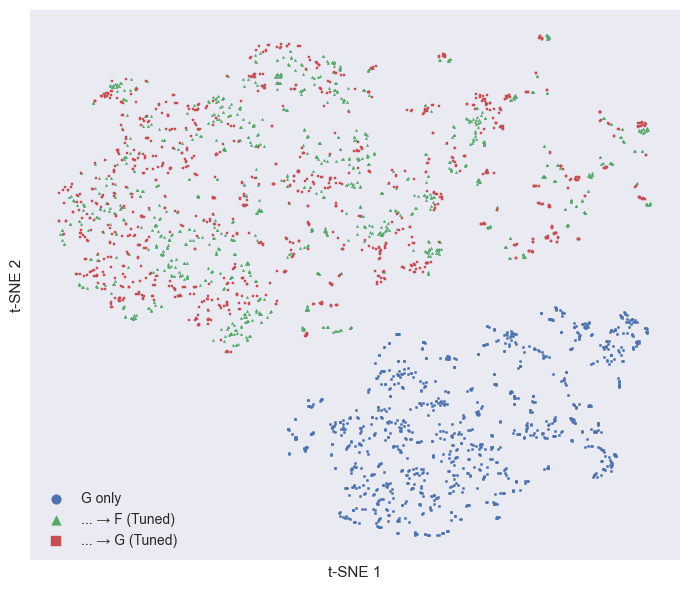
\includegraphics[width=\textwidth]{images/experiments/tuned-tsne-regg-outofdist.png}
        \caption{Regulation \textbf{G}, out-of-distribution ($n=1012$).}
        \label{fig:tsne-tuned-regg-outdist}
    \end{subfigure}
    \caption{t-SNE visualization of action logits of tuned agents for every observation. Letters represent the regulation the agent is trained or fine-tuned on (e.g. ``$... \rightarrow \text{F}$" is fine-tuned from regulation \textbf{A} to \textbf{B} to ... to \textbf{F}).}
    \label{fig:tsne-tuned}
\end{figure}

\begin{figure}[ht]
    \centering
    \begin{subfigure}{.5\textwidth}
        \centering
        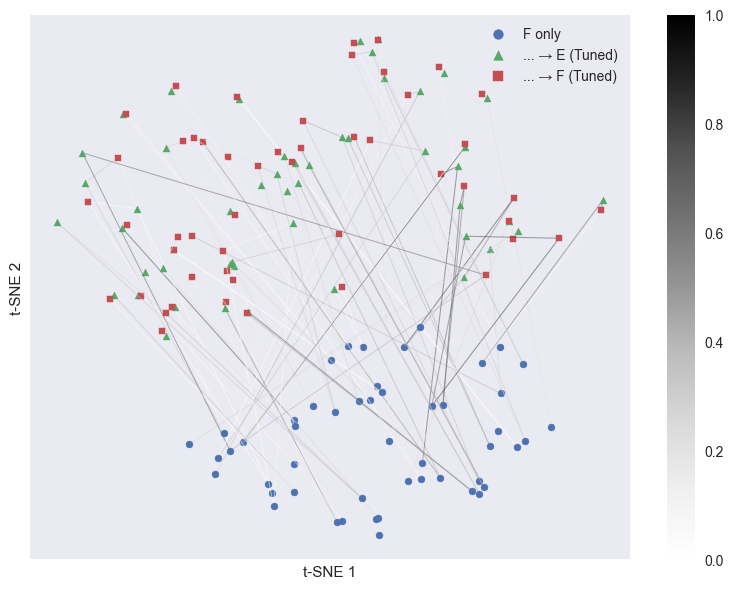
\includegraphics[width=\textwidth]{images/experiments/tuned-tsne-regf-indist-lines.png}
        \caption{Regulation \textbf{F}, in-distribution ($n=924$).}
        \label{fig:tsne-tuned-lines-regf-indist}
    \end{subfigure}%
    \begin{subfigure}{.5\textwidth}
        \centering
        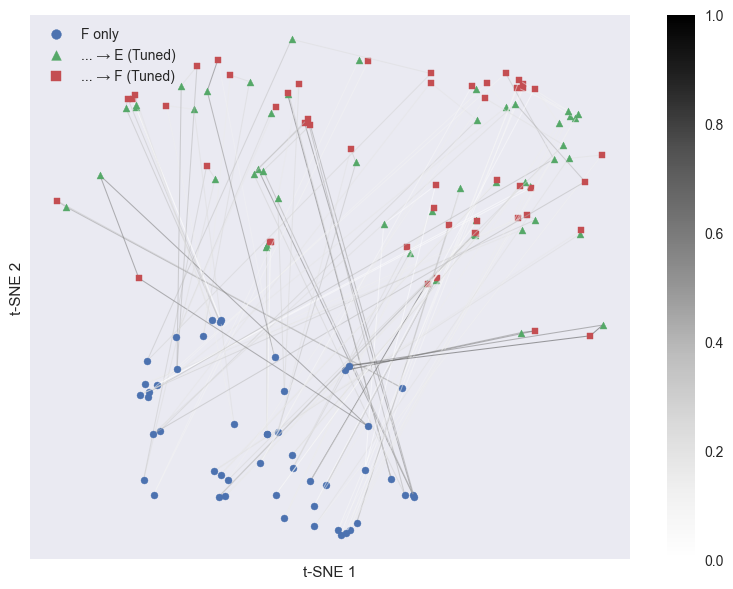
\includegraphics[width=\textwidth]{images/experiments/tuned-tsne-regf-outofdist-lines.png}
        \caption{Regulation \textbf{F}, out-of-distribution ($n=1021$).}
        \label{fig:tsne-tuned-lines-regf-outdist}
    \end{subfigure}
    \vskip\baselineskip
    \begin{subfigure}{.5\textwidth}
        \centering
        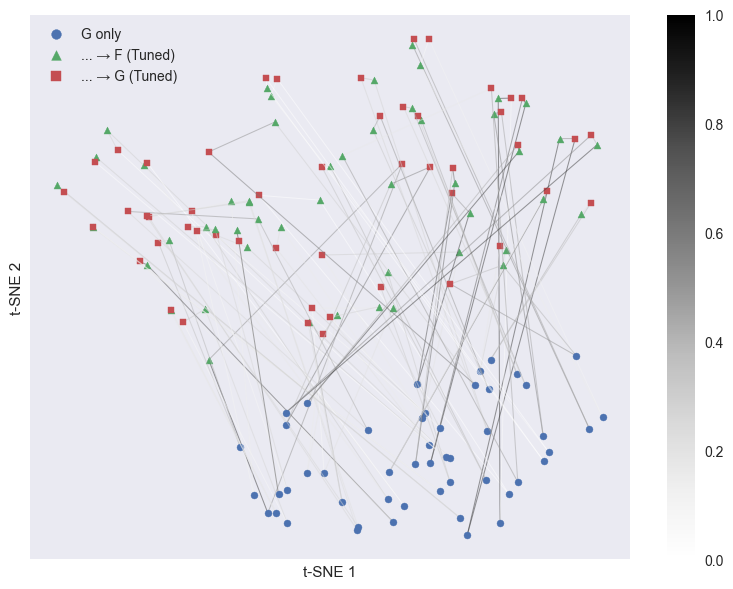
\includegraphics[width=\textwidth]{images/experiments/tuned-tsne-regg-indist-lines.png}
        \caption{Regulation \textbf{G}, in-distribution ($n=1041$).}
        \label{fig:tsne-tuned-lines-regg-indist}
    \end{subfigure}%
    \begin{subfigure}{.5\textwidth}
        \centering
        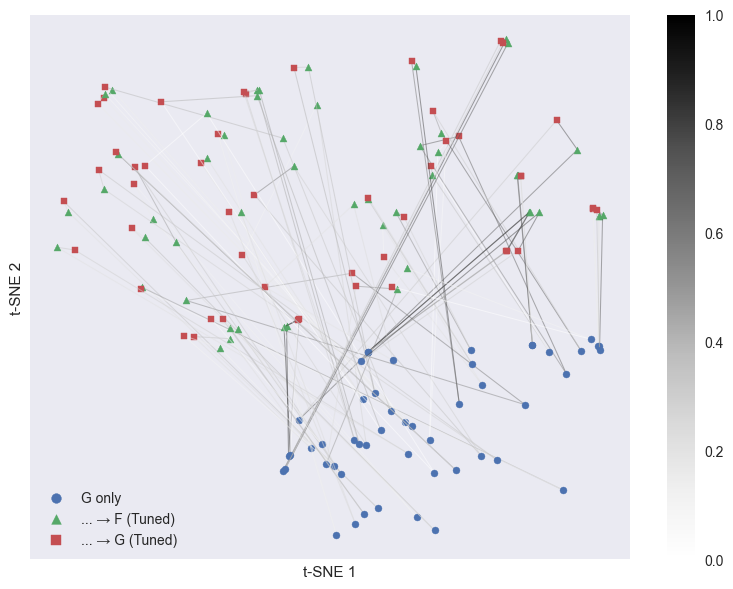
\includegraphics[width=\textwidth]{images/experiments/tuned-tsne-regg-outofdist-lines.png}
        \caption{Regulation \textbf{G}, out-of-distribution ($n=1012$).}
        \label{fig:tsne-tuned-lines-regg-outdist}
    \end{subfigure}
    \caption{t-SNE visualization of action logits of tuned agents for 50 sampled observations. Letters represent the regulation the agent is trained or fine-tuned on (e.g. ``$... \rightarrow \text{F}$" is fine-tuned from regulation \textbf{A} to \textbf{B} to ... to \textbf{F}). Lines connect points showing the same observation, and are colored according to the Jensen-Shannon distance between the respective action probabilities.}
    \label{fig:tsne-tuned-lines}
\end{figure}
